\documentclass[11pt,landscape]{exam}
\usepackage[margin=0.3in]{geometry}
\usepackage{multicol,tikz,graphicx}
\usetikzlibrary{shadings,decorations.pathmorphing,arrows.meta,patterns}




\begin{document}

\newcommand{\content}{


}

\begin{multicols}{2}

  \noindent
  An image is the point where light rays \fillin[intersect][15em].

  \vspace{1em}

  \noindent
  \begin{tabular}{p{2.1in}p{0.1in}p{2.1in}}
    \textbf{virtual images} &&  \textbf{real images} \\\\
    %
    rays of light appear to intersect at a location, but in reality there is \fillin[no light][6.5em] there.
    %
    &&
    rays of light  do \hfill \fillin[intersect][7em] at a point in space \\\\
    \fillin[cannot be][8em] focused on a screen &&
    \fillin[can be][8em] focused on a screen
    
  \end{tabular}

  \vspace{8em}

  \subsection*{Equations for Locating Images}

  \vspace{2em}
  
  \hfill

  Thin Lens Equation:

  \vspace{3em}

  Mangification Equation:

  \vspace{2em}


  \subsection*{Variables \& Sign Conventions}

  \renewcommand{\arraystretch}{2}

  \begin{tabular}{cll}
  $d_o$ & distance between lens and object \\
  $d_i$ & distance between lens and image \\
  $f$   & focal length \\ 
  $h_o$ & height of object \\
  $h_i$ & height of image \\
  $m$   & magnification \\
  \end{tabular}


\columnbreak

\noindent
Consider a ray of light hitting glass:
  
  \begin{center}
    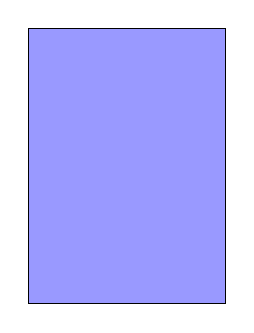
\begin{tikzpicture}
        \draw[fill=blue!40] (0,0) rectangle (2.5,3.5);
    \end{tikzpicture}
  \end{center}

\noindent
Now, how could we shape a piece of glass to manipulate the direction of light?
  
  \begin{center}
    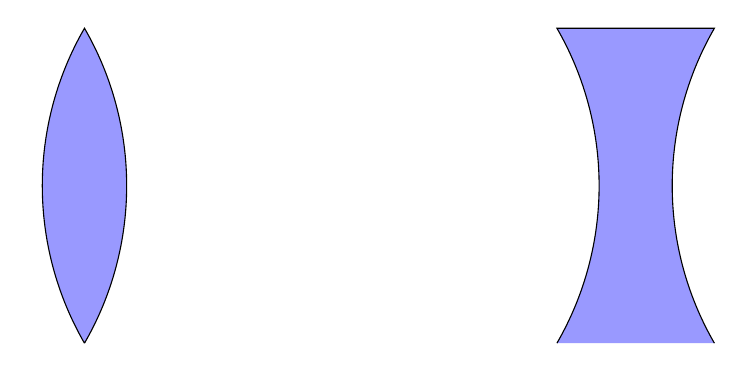
\begin{tikzpicture}
      \draw[fill=blue!40] (0,0) 
        arc (-30:30:4) 
        arc (150:210:4);

      \draw[fill=blue!40] (6,0) 
        arc (-30:30:4) --
        ++(2,0)
        arc (150:210:4);
    \end{tikzpicture}
  \end{center}

  \vspace*{4em}


\noindent
How about curved mirrors?  How could we shape them to manipulate the direction of light?
  
  \begin{center}
    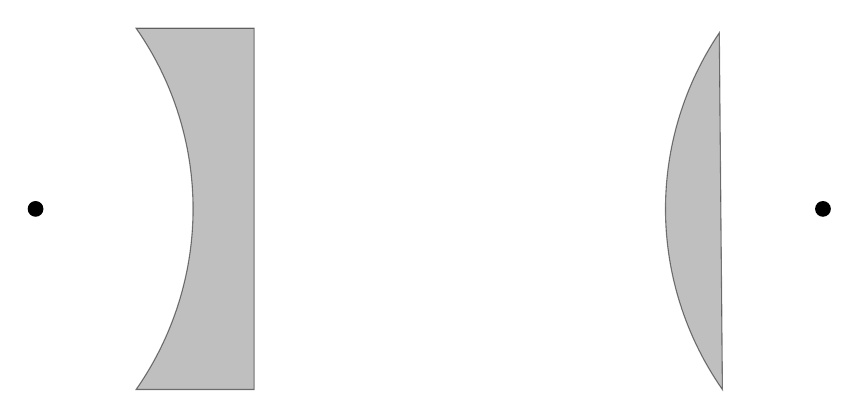
\begin{tikzpicture}
      \def\radius{4}
      \def\angwidth{35}
      \begin{scope}[shift={(14,0)}]
        \draw[fill=gray,semitransparent] (-\radius,0) 
          arc (180:146:\radius)
          -- (215:\radius)
          arc (215:180:\radius)
          -- cycle; 
        \fill (-0.5*\radius,0) circle (0.1);
      \end{scope}
      \begin{scope}
        \draw[fill=gray,semitransparent] (\radius,0) 
          arc (0:\angwidth:\radius) --
          ++(1.5,0) |- (-\angwidth:\radius)
          arc (-\angwidth:0:\radius)
          -- cycle;  
        \fill (0.5*\radius,0) circle (0.1);
      \end{scope}
    \end{tikzpicture}
  \end{center}

  \vspace*{2em}


\end{multicols}

\end{document}